 \documentclass{beamer}

\usetheme{MagdeburgFIN}
\usefonttheme{structurebold}
\usepackage{graphicx}
\usepackage{float}
\usepackage{url}
\usepackage{pdfpages}
\usepackage[utf8]{inputenc}
\usepackage{tikz}


\title{Exposé: Wireless Ranging in Swarm Robotics}
\author{Sebastian Mai}
\date{03. 12. 2015}
%\institute{Student Conference on Software Engineering and Database Systems}

\begin{document}

\begin{frame}[plain]
 \titlepage
\end{frame}



\section[Agenda]{}
\begin{frame}
	\frametitle{Agenda}
	\tableofcontents
\end{frame}

\section{Motivation}
\begin{frame}
	\frametitle{Motivation}
	\framesubtitle{Problem}
	\begin{columns}
		\column{.4\textwidth}
		\begin{figure}
			\centering
			\includegraphics[width=0.9\textwidth]{img/copter.png}
			\caption{FINken 3 Roboter}
		\end{figure}
		\column{.6\textwidth}
		\begin{itemize}
			\item Ziel: Schwarmverhalten auf Fliegenden Robotern
			\item Aber: Schwarmverhalten basiert oft auf Distanzfunktion
			\item Mögliche Quellen für Distanzen: Abstands Sensoren, Ranging
		\end{itemize}
	\end{columns}
\end{frame}

\begin{frame}
	\frametitle{Motivation}
	\framesubtitle{Ranging Node$\leftrightarrow$Enviroment}
	Entfernungswerte der Ultraschallsensoren
	\begin{itemize}
		\item Keine Unterscheidung zwischen Umgebung und Schwarm
		\item Entfernugsmessewerte $\neq$ Mathematische Distanz
		\item Mehrere Distanzen für eine Dimension
	\end{itemize}
\end{frame}
\begin{frame}
	\frametitle{Motivation}
	\framesubtitle{Ranging Node$\leftrightarrow$Node}
	\begin{itemize}
		\item Messung Addressbasiert
		\item Entferungsmesswerte ähnlich zu Mathematischer Distanz
		\item Distanz ist eindimensional
	\end{itemize}
\end{frame}

\section{Ranging – Prior Art}
\begin{frame}
	\frametitle{Ranging – Prior Art}
	\framesubtitle{Abgrenzung}
	\begin{itemize}
		\item Sensor misst physikalischen Abstand
		\item Messung von Knoten zu Knoten
		\item Anwendung von Ranging Hardware ist fast ausschließlich Postitionsbestimmung
		\item Anwendung im Schwarm: Distanzen zwischen Individuen, oder Anchor-Nodes
	\end{itemize}
\end{frame}

\begin{frame}
	\frametitle{Ranging – Prior Art}
	\framesubtitle{Anforderungen}
	\begin{itemize}
		\item In Copter integrierbar 
		\item Interaktion zwischen Copter und Sensoren minimal
		\item Brauchbare Entfernungsmessung
	\end{itemize}
\end{frame}

\begin{frame}
	\frametitle{Ranging — Prior Art}
	\framesubtitle{Technologien}
	\begin{itemize}
		\item Optisches Tracking - extern, teuer
		\item Ultraschallbasiertes Ranging - interagiert mit Ultraschall-Sensoren
		\item RSSI-Ranging - unpräziese, richtungsabhängig
	\end{itemize}
	\begin{itemize}
		\item Time-of-Flight-Ranging - Dekawave
		\item Phasendifferenzmessung - ATMEL-RTB
	\end{itemize}
\end{frame}

\section{Konzept}
\begin{frame}
	\frametitle{Konzept}
	\framesubtitle{Kommunikation}
	
\begin{description}
	\item[ Idee ] Ranging-API über Sensorbus verfügbar machen.
	\item[ Interface ] Messung auslösen und Messwerte Abfragen per I2C
	\item[ Hardware ] Integration mit anderer Hardware der Selben Technologie
\end{description}
\end{frame}

\section{Messreihen und Evaluation}
\begin{frame}
	\frametitle{Messreihen und Evaluation}
	\framesubtitle{Ziele der Evaluation}
	Ziel der Evaluation
	\begin{itemize}
		\item Funkstörungen
		\item Zusammenhang Distanz-Messwert
		\item Einfluss von Drehung
		\item Eigenschaften eines Distanzmaßes
	\end{itemize}

\end{frame}

\begin{frame}
	\frametitle{Messreihen und Evaluation}
	\framesubtitle{Funkstörungen}

	\begin{columns}
		\column{ .4\textwidth }

		\begin{figure}
			\centering
			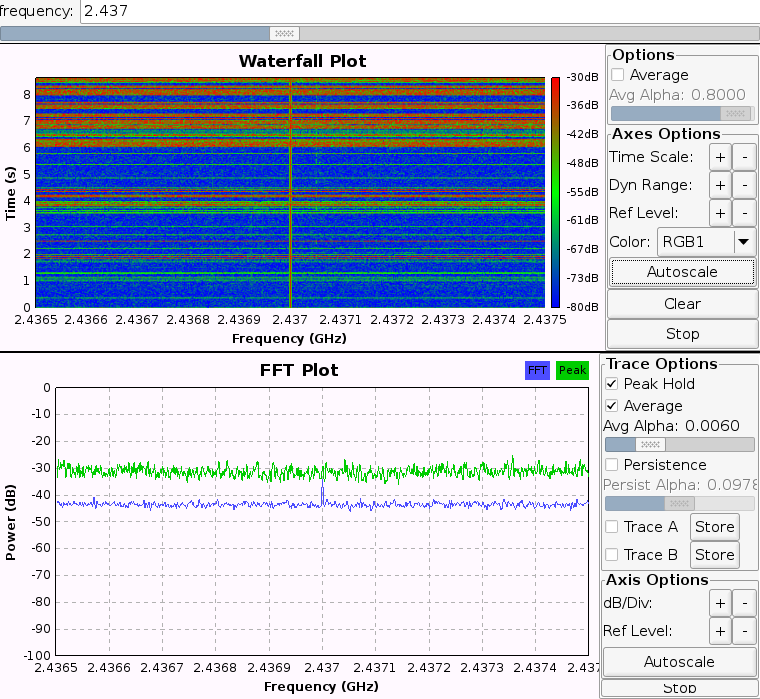
\includegraphics[width=0.9\textwidth]{img/ch6.png}
			\caption{Funkspektrum 2.437GHz}
		\end{figure}
		\column{ .6\textwidth }
		\begin{itemize}
			\item Schwer quantifizierbar – dafür wäre andere Hardware nötig.
			\item Finden eines wenig Benutzen Frequenzbereiches mit SDR soll Einfluss von Funkstörungen verringen
			\item Messungen während guter Bedingungen
			\item Fernbedienungslink verursacht starke Störungen
		\end{itemize}

	\end{columns}	


\end{frame}

\begin{frame}
	\frametitle{Messreihen und Evaluation}
	\framesubtitle{Zussammenhang Distanz – Messwert}
	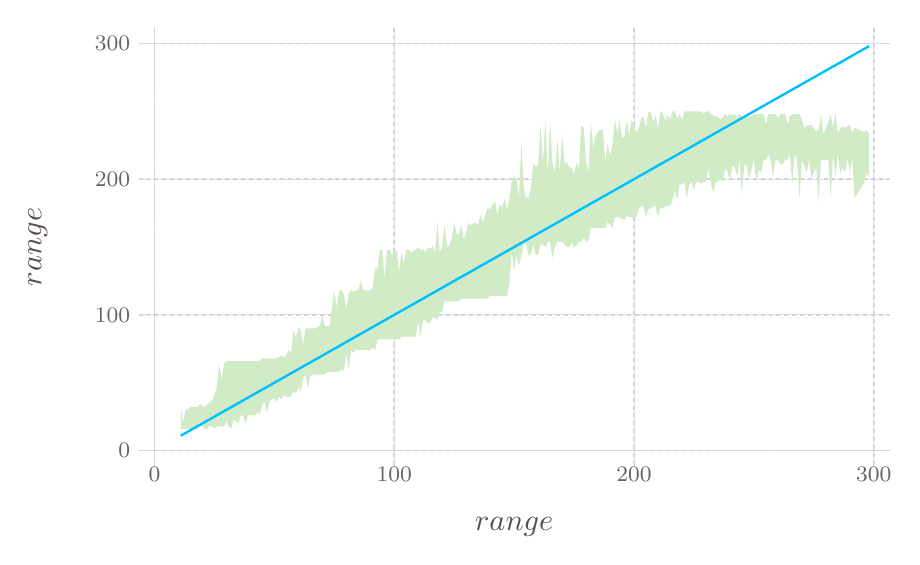
\begin{tikzpicture}[x=1mm,y=-1mm]
\definecolor{mycolor000000}{rgb}{0,0,0}
\definecolor{mycolor000000}{rgb}{0,0,0}
\definecolor{mycolorD0D0E0}{rgb}{0.82,0.82,0.88}
\definecolor{mycolorD1EAC7}{rgb}{0.82,0.92,0.78}
\definecolor{mycolor6C606B}{rgb}{0.42,0.38,0.42}
\definecolor{mycolor564A55}{rgb}{0.34,0.29,0.33}
\definecolor{mycolor00BFFF}{rgb}{0,0.75,1}
\begin{scope}
\begin{scope}
\draw (67.32,68.39) node [text=mycolor564A55,draw=mycolor000000,draw opacity=0,rotate around={-0: (0,1.81)},inner sep=0.0]{\fontsize{3.88mm}{4.66mm}\selectfont $\text{range}$};
\end{scope}
\begin{scope}
\draw (21.63,61.72) node [text=mycolor6C606B,rotate around={-0: (45.68,1.34)},inner sep=0.0]{\fontsize{2.82mm}{3.39mm}\selectfont $\text{0}$};
\draw (52.09,61.72) node [text=mycolor6C606B,rotate around={-0: (15.23,1.34)},inner sep=0.0]{\fontsize{2.82mm}{3.39mm}\selectfont $\text{100}$};
\draw (82.54,61.72) node [text=mycolor6C606B,rotate around={-0: (-15.23,1.34)},inner sep=0.0]{\fontsize{2.82mm}{3.39mm}\selectfont $\text{200}$};
\draw (113,61.72) node [text=mycolor6C606B,rotate around={-0: (-45.68,1.34)},inner sep=0.0]{\fontsize{2.82mm}{3.39mm}\selectfont $\text{300}$};
\end{scope}
\begin{scope}
\clip  (19.63,5) -- (115,5) -- (115,60.72) -- (19.63,60.72);
\begin{scope}
\clip  (19.63,5) -- (115,5) -- (115,60.72) -- (19.63,60.72);
\path [fill=mycolor000000,fill opacity=0,draw=mycolor000000,draw opacity=0] (19.63,5) rectangle +(95.37,55.72);
\end{scope}
\begin{scope}
[dash pattern=on 0.5mm off 0.5mm,line width=0.2mm]
\path [fill=mycolor000000,draw=mycolorD0D0E0]  (19.63,58.71) -- (115,58.71);
\path [fill=mycolor000000,draw=mycolorD0D0E0]  (19.63,41.48) -- (115,41.48);
\path [fill=mycolor000000,draw=mycolorD0D0E0]  (19.63,24.24) -- (115,24.24);
\path [fill=mycolor000000,draw=mycolorD0D0E0]  (19.63,7) -- (115,7);
\end{scope}
\begin{scope}
[dash pattern=on 0.5mm off 0.5mm,line width=0.2mm]
\path [fill=mycolor000000,draw=mycolorD0D0E0]  (21.63,5) -- (21.63,60.72);
\path [fill=mycolor000000,draw=mycolorD0D0E0]  (52.09,5) -- (52.09,60.72);
\path [fill=mycolor000000,draw=mycolorD0D0E0]  (82.54,5) -- (82.54,60.72);
\path [fill=mycolor000000,draw=mycolorD0D0E0]  (113,5) -- (113,60.72);
\end{scope}
\begin{scope}
\begin{scope}
[line width=0.3mm]
\path [fill=mycolorD1EAC7,draw=mycolor000000,draw opacity=0]  (112.39,24.07) -- (112.09,23.38) -- (111.78,24.67) -- (110.56,26.65) -- (110.26,21.64) -- (109.95,23.34) -- (109.65,21.57) -- (109.35,23.38) -- (109.04,22.79) -- (108.74,23.48) -- (108.43,21.14) -- (108.13,23.89) -- (107.82,21.24) -- (107.52,26.67) -- (107.21,21.82) -- (106.6,21.82) -- (106.3,21.82) -- (106,27) -- (105.69,22.79) -- (105.39,23.38) -- (105.08,24.32) -- (104.78,21.82) -- (104.47,23.29) -- (104.17,22.6) -- (103.86,21.82) -- (103.56,26.65) -- (103.25,21.82) -- (102.95,21.08) -- (102.64,24.84) -- (102.34,21.14) -- (102.04,21.82) -- (101.73,21.82) -- (101.43,22.34) -- (101.12,22.31) -- (100.82,21.82) -- (100.51,21.82) -- (100.21,23.89) -- (99.9,21.82) -- (99.6,21.14) -- (99.29,21.82) -- (98.99,21.82) -- (98.69,23.41) -- (98.38,23.1) -- (98.08,24.58) -- (97.77,21.82) -- (97.47,22.98) -- (97.16,24.2) -- (96.86,22.45) -- (96.55,22.39) -- (96.25,26.24) -- (95.94,21.82) -- (95.64,23.89) -- (95.34,22.69) -- (95.03,22.51) -- (94.73,24.58) -- (94.42,23.27) -- (94.12,22.86) -- (93.81,24.58) -- (93.51,24.13) -- (93.2,24.58) -- (92.9,24.58) -- (92.59,25.96) -- (92.29,24.7) -- (91.99,22.86) -- (91.68,24.58) -- (91.38,24.58) -- (91.07,24.79) -- (90.77,24.58) -- (90.46,24.58) -- (90.16,25.53) -- (89.85,24.58) -- (89.55,24.93) -- (89.24,26.74) -- (88.94,24.58) -- (88.64,24.93) -- (88.33,24.93) -- (88.03,26.79) -- (87.72,25.7) -- (87.42,26.93) -- (87.11,27.67) -- (86.81,27.6) -- (86.5,27.69) -- (86.2,28.03) -- (85.89,27.75) -- (85.59,29.07) -- (85.28,27.69) -- (84.98,27.7) -- (84.68,27.93) -- (84.37,28) -- (84.07,29.07) -- (83.76,27.69) -- (83.46,27.69) -- (83.15,28.03) -- (82.85,29.07) -- (82.54,29.07) -- (82.24,29.07) -- (81.93,29.07) -- (81.63,28.91) -- (81.33,29.41) -- (81.02,29.34) -- (80.72,29.07) -- (80.41,29.07) -- (80.11,29.07) -- (79.8,30.44) -- (79.5,30.06) -- (79.19,29.67) -- (78.89,30.44) -- (78.58,30.44) -- (78.28,30.44) -- (77.98,30.44) -- (77.67,30.44) -- (77.37,30.44) -- (77.06,30.44) -- (76.76,32.1) -- (76.45,32.17) -- (76.15,31.65) -- (75.84,32.17) -- (75.54,32.17) -- (75.23,32.65) -- (74.93,32.86) -- (74.63,32.32) -- (74.32,32.86) -- (74.02,32.86) -- (73.71,32.51) -- (73.41,32.17) -- (73.1,32.17) -- (72.8,32.17) -- (72.49,32.86) -- (72.19,34.24) -- (71.88,32.17) -- (71.58,32.17) -- (71.28,32.86) -- (70.97,32.6) -- (70.67,32.44) -- (70.36,33.89) -- (70.06,33.89) -- (69.75,32.48) -- (69.45,33.82) -- (69.14,33.84) -- (68.84,32.51) -- (68.53,32.37) -- (68.23,33.93) -- (67.92,35.27) -- (67.62,33.89) -- (67.32,35.96) -- (67.01,33.46) -- (66.71,37.51) -- (66.4,39.06) -- (66.1,39.06) -- (65.79,39.06) -- (65.49,39.06) -- (65.18,39.06) -- (64.88,39.06) -- (64.57,39.06) -- (64.27,39.06) -- (63.97,39.41) -- (63.66,39.41) -- (63.36,39.41) -- (63.05,39.41) -- (62.75,39.41) -- (62.44,39.41) -- (62.14,39.41) -- (61.83,39.41) -- (61.53,39.41) -- (61.22,39.41) -- (60.92,39.41) -- (60.62,39.41) -- (60.31,39.72) -- (60.01,39.75) -- (59.7,39.75) -- (59.4,39.75) -- (59.09,39.75) -- (58.79,39.75) -- (58.48,39.75) -- (58.18,41.13) -- (57.87,41.08) -- (57.57,42.17) -- (57.27,41.82) -- (56.96,41.82) -- (56.66,42.51) -- (56.35,42.51) -- (56.05,42.17) -- (55.74,42.17) -- (55.44,44.23) -- (55.13,42.34) -- (54.83,44.23) -- (54.52,44.23) -- (54.22,44.23) -- (53.92,44.23) -- (53.61,44.23) -- (53.31,44.23) -- (53,44.23) -- (52.7,44.58) -- (52.39,44.58) -- (52.09,44.58) -- (51.78,44.58) -- (51.48,44.58) -- (51.17,44.58) -- (50.87,44.58) -- (50.56,44.58) -- (50.26,44.58) -- (49.96,44.75) -- (49.65,45.96) -- (49.35,45.61) -- (49.04,45.96) -- (48.74,45.96) -- (48.43,45.96) -- (48.13,45.96) -- (47.82,45.96) -- (47.52,45.96) -- (47.21,45.96) -- (46.91,46.3) -- (46.61,45.96) -- (46.3,48.37) -- (46,46.3) -- (45.69,48.65) -- (45.39,48.39) -- (45.08,48.72) -- (44.78,48.72) -- (44.47,48.72) -- (44.17,48.72) -- (43.86,48.72) -- (43.56,48.72) -- (43.26,49.06) -- (42.95,49.06) -- (42.65,49.06) -- (42.34,49.06) -- (42.04,49.06) -- (41.73,49.06) -- (41.43,49.25) -- (41.12,50.85) -- (40.82,49.06) -- (40.51,49.56) -- (40.21,51.13) -- (39.91,50.68) -- (39.6,51.47) -- (39.3,51.13) -- (38.99,51.82) -- (38.69,51.96) -- (38.38,51.87) -- (38.08,51.63) -- (37.77,52.16) -- (37.47,51.82) -- (37.16,52.51) -- (36.86,52.16) -- (36.56,52.16) -- (36.25,52.51) -- (35.95,53.89) -- (35.64,52.51) -- (35.34,52.85) -- (35.03,54.11) -- (34.73,53.89) -- (34.42,54.23) -- (34.12,54.25) -- (33.81,54.23) -- (33.51,54.23) -- (33.2,55.27) -- (32.9,54.27) -- (32.6,54.23) -- (32.29,55.27) -- (31.99,54.92) -- (31.68,54.84) -- (31.38,55.96) -- (31.07,55.61) -- (30.77,54.92) -- (30.46,55.7) -- (30.16,55.61) -- (29.85,55.61) -- (29.55,55.61) -- (29.25,55.96) -- (28.94,55.61) -- (28.64,55.61) -- (28.33,55.96) -- (28.03,55.96) -- (27.72,55.61) -- (27.42,55.61) -- (27.11,55.96) -- (26.81,55.96) -- (26.5,55.96) -- (26.2,55.96) -- (25.9,55.96) -- (25.59,55.96) -- (25.29,55.96) -- (24.98,55.96) -- (24.98,53.2) -- (25.29,55.22) -- (25.59,53.47) -- (25.9,53.54) -- (26.2,53.2) -- (26.5,53.2) -- (26.81,53.2) -- (27.11,53.2) -- (27.42,52.79) -- (27.72,53.04) -- (28.03,53.2) -- (28.33,52.85) -- (28.64,52.6) -- (28.94,52.44) -- (29.25,51.65) -- (29.55,50.65) -- (29.85,47.68) -- (30.16,49.75) -- (30.46,47.68) -- (30.77,47.34) -- (31.07,47.34) -- (31.38,47.34) -- (31.68,47.34) -- (31.99,47.34) -- (32.29,47.34) -- (32.6,47.34) -- (32.9,47.34) -- (33.2,47.34) -- (33.51,47.34) -- (33.81,47.34) -- (34.12,47.34) -- (34.42,47.34) -- (34.73,47.34) -- (35.03,47.34) -- (35.34,46.99) -- (35.64,46.99) -- (35.95,46.99) -- (36.25,46.99) -- (36.56,46.99) -- (36.86,46.99) -- (37.16,46.99) -- (37.47,46.8) -- (37.77,46.65) -- (38.08,46.84) -- (38.38,46.6) -- (38.69,45.89) -- (38.99,46.3) -- (39.3,43.42) -- (39.6,44.23) -- (39.91,43.2) -- (40.21,43.2) -- (40.51,45.27) -- (40.82,43.2) -- (41.12,43.2) -- (41.43,43.2) -- (41.73,43.2) -- (42.04,43.2) -- (42.34,43.01) -- (42.65,42.86) -- (42.95,41.51) -- (43.26,42.86) -- (43.56,42.86) -- (43.86,42.86) -- (44.17,40.68) -- (44.47,38.37) -- (44.78,40.55) -- (45.08,38.37) -- (45.39,38.37) -- (45.69,38.79) -- (46,40.79) -- (46.3,38.72) -- (46.61,38.37) -- (46.91,38.55) -- (47.21,38.37) -- (47.52,38.37) -- (47.82,37.13) -- (48.13,38.37) -- (48.43,38.37) -- (48.74,38.37) -- (49.04,38.37) -- (49.35,38.03) -- (49.65,35.56) -- (49.96,35.62) -- (50.26,33.2) -- (50.56,33.2) -- (50.87,36.93) -- (51.17,33.2) -- (51.48,33.2) -- (51.78,33.89) -- (52.09,33.2) -- (52.39,33.2) -- (52.7,35.96) -- (53,33.55) -- (53.31,35) -- (53.61,33.2) -- (53.92,33.2) -- (54.22,33.55) -- (54.52,33.32) -- (54.83,33.2) -- (55.13,32.86) -- (55.44,33.29) -- (55.74,33.1) -- (56.05,33.55) -- (56.35,32.94) -- (56.66,33.08) -- (56.96,32.74) -- (57.27,33.55) -- (57.57,29.69) -- (57.87,33.55) -- (58.18,32.86) -- (58.48,30.05) -- (58.79,32.86) -- (59.09,32.72) -- (59.4,31.74) -- (59.7,29.75) -- (60.01,31.22) -- (60.31,31.24) -- (60.62,30.1) -- (60.92,31.82) -- (61.22,31.03) -- (61.53,29.75) -- (61.83,30.1) -- (62.14,29.82) -- (62.44,29.75) -- (62.75,30.1) -- (63.05,28.72) -- (63.36,29.75) -- (63.66,28.72) -- (63.97,27.86) -- (64.27,28.17) -- (64.57,27.43) -- (64.88,27) -- (65.18,28.72) -- (65.49,27.34) -- (65.79,27.86) -- (66.1,26.62) -- (66.4,28.1) -- (66.71,26.62) -- (67.01,24.58) -- (67.32,23.82) -- (67.62,24.24) -- (67.92,26.82) -- (68.23,19.45) -- (68.53,25.27) -- (68.84,26.65) -- (69.14,26.65) -- (69.45,25.31) -- (69.75,22.24) -- (70.06,22.65) -- (70.36,22.38) -- (70.67,17.48) -- (70.97,22.17) -- (71.28,16.64) -- (71.58,23.55) -- (71.88,16.72) -- (72.19,22.27) -- (72.49,23.51) -- (72.8,19.19) -- (73.1,23.43) -- (73.41,18.45) -- (73.71,22.17) -- (74.02,22.08) -- (74.32,22.72) -- (74.63,22.74) -- (74.93,23.55) -- (75.23,22.17) -- (75.54,22.86) -- (75.84,17.41) -- (76.15,17.69) -- (76.45,22.17) -- (76.76,23.2) -- (77.06,16.81) -- (77.37,20.45) -- (77.67,18.65) -- (77.98,18.24) -- (78.28,18.03) -- (78.58,17.91) -- (78.89,22.17) -- (79.19,19.67) -- (79.5,21.24) -- (79.8,19.89) -- (80.11,16.65) -- (80.41,18.41) -- (80.72,16.81) -- (81.02,19.07) -- (81.33,18.79) -- (81.63,16.65) -- (81.93,18.72) -- (82.24,16.65) -- (82.54,17.48) -- (82.85,18.31) -- (83.15,17.76) -- (83.46,16.38) -- (83.76,16.43) -- (84.07,17.69) -- (84.37,15.69) -- (84.68,15.72) -- (84.98,17) -- (85.28,16.19) -- (85.59,17.77) -- (85.89,15.62) -- (86.2,15.93) -- (86.5,16.79) -- (86.81,16.14) -- (87.11,16.65) -- (87.42,15.62) -- (87.72,15.62) -- (88.03,16.45) -- (88.33,15.96) -- (88.64,16.69) -- (88.94,15.62) -- (89.24,15.62) -- (89.55,15.62) -- (89.85,15.62) -- (90.16,15.62) -- (90.46,15.62) -- (90.77,15.62) -- (91.07,15.62) -- (91.38,15.96) -- (91.68,15.62) -- (91.99,15.62) -- (92.29,15.96) -- (92.59,16.14) -- (92.9,16.31) -- (93.2,16.31) -- (93.51,16.65) -- (93.81,16.39) -- (94.12,15.96) -- (94.42,16.31) -- (94.73,15.96) -- (95.03,16.12) -- (95.34,15.96) -- (95.64,16.31) -- (95.94,15.96) -- (96.25,16.31) -- (96.55,16.31) -- (96.86,16.31) -- (97.16,16.31) -- (97.47,16.19) -- (97.77,15.96) -- (98.08,15.96) -- (98.38,15.96) -- (98.69,15.96) -- (98.99,15.96) -- (99.29,17.34) -- (99.6,15.96) -- (99.9,15.96) -- (100.21,15.96) -- (100.51,15.96) -- (100.82,16.46) -- (101.12,15.96) -- (101.43,15.96) -- (101.73,15.96) -- (102.04,17.31) -- (102.34,16.27) -- (102.64,15.96) -- (102.95,15.96) -- (103.25,16.03) -- (103.56,15.96) -- (103.86,16.72) -- (104.17,17.72) -- (104.47,17.45) -- (104.78,17.39) -- (105.08,17.34) -- (105.39,17.83) -- (105.69,18.17) -- (106,17.89) -- (106.3,15.96) -- (106.6,18.55) -- (107.21,17) -- (107.52,15.96) -- (107.82,17.72) -- (108.13,15.96) -- (108.43,18.38) -- (108.74,17.89) -- (109.04,17.55) -- (109.35,17.69) -- (109.65,17.52) -- (109.95,17.21) -- (110.26,18.38) -- (110.56,17.69) -- (111.78,18.29) -- (112.09,18.03) -- (112.39,18.38) -- cycle;
\end{scope}
\begin{scope}
[line width=0.3mm]
\path [fill=mycolor000000,fill opacity=0,draw=mycolor00BFFF]  (24.98,56.82) -- (25.29,56.65) -- (25.59,56.47) -- (25.9,56.3) -- (26.2,56.13) -- (26.5,55.96) -- (26.81,55.78) -- (27.11,55.61) -- (27.42,55.44) -- (27.72,55.27) -- (28.03,55.09) -- (28.33,54.92) -- (28.64,54.75) -- (28.94,54.58) -- (29.25,54.41) -- (29.55,54.23) -- (29.85,54.06) -- (30.16,53.89) -- (30.46,53.72) -- (30.77,53.54) -- (31.07,53.37) -- (31.38,53.2) -- (31.68,53.03) -- (31.99,52.85) -- (32.29,52.68) -- (32.6,52.51) -- (32.9,52.34) -- (33.2,52.16) -- (33.51,51.99) -- (33.81,51.82) -- (34.12,51.65) -- (34.42,51.47) -- (34.73,51.3) -- (35.03,51.13) -- (35.34,50.96) -- (35.64,50.79) -- (35.95,50.61) -- (36.25,50.44) -- (36.56,50.27) -- (36.86,50.1) -- (37.16,49.92) -- (37.47,49.75) -- (37.77,49.58) -- (38.08,49.41) -- (38.38,49.23) -- (38.69,49.06) -- (38.99,48.89) -- (39.3,48.72) -- (39.6,48.54) -- (39.91,48.37) -- (40.21,48.2) -- (40.51,48.03) -- (40.82,47.85) -- (41.12,47.68) -- (41.43,47.51) -- (41.73,47.34) -- (42.04,47.17) -- (42.34,46.99) -- (42.65,46.82) -- (42.95,46.65) -- (43.26,46.48) -- (43.56,46.3) -- (43.86,46.13) -- (44.17,45.96) -- (44.47,45.79) -- (44.78,45.61) -- (45.08,45.44) -- (45.39,45.27) -- (45.69,45.1) -- (46,44.92) -- (46.3,44.75) -- (46.61,44.58) -- (46.91,44.41) -- (47.21,44.23) -- (47.52,44.06) -- (47.82,43.89) -- (48.13,43.72) -- (48.43,43.55) -- (48.74,43.37) -- (49.04,43.2) -- (49.35,43.03) -- (49.65,42.86) -- (49.96,42.68) -- (50.26,42.51) -- (50.56,42.34) -- (50.87,42.17) -- (51.17,41.99) -- (51.48,41.82) -- (51.78,41.65) -- (52.09,41.48) -- (52.39,41.3) -- (52.7,41.13) -- (53,40.96) -- (53.31,40.79) -- (53.61,40.61) -- (53.92,40.44) -- (54.22,40.27) -- (54.52,40.1) -- (54.83,39.93) -- (55.13,39.75) -- (55.44,39.58) -- (55.74,39.41) -- (56.05,39.24) -- (56.35,39.06) -- (56.66,38.89) -- (56.96,38.72) -- (57.27,38.55) -- (57.57,38.37) -- (57.87,38.2) -- (58.18,38.03) -- (58.48,37.86) -- (58.79,37.68) -- (59.09,37.51) -- (59.4,37.34) -- (59.7,37.17) -- (60.01,36.99) -- (60.31,36.82) -- (60.62,36.65) -- (60.92,36.48) -- (61.22,36.31) -- (61.53,36.13) -- (61.83,35.96) -- (62.14,35.79) -- (62.44,35.62) -- (62.75,35.44) -- (63.05,35.27) -- (63.36,35.1) -- (63.66,34.93) -- (63.97,34.75) -- (64.27,34.58) -- (64.57,34.41) -- (64.88,34.24) -- (65.18,34.06) -- (65.49,33.89) -- (65.79,33.72) -- (66.1,33.55) -- (66.4,33.37) -- (66.71,33.2) -- (67.01,33.03) -- (67.32,32.86) -- (67.62,32.69) -- (67.92,32.51) -- (68.23,32.34) -- (68.53,32.17) -- (68.84,32) -- (69.14,31.82) -- (69.45,31.65) -- (69.75,31.48) -- (70.06,31.31) -- (70.36,31.13) -- (70.67,30.96) -- (70.97,30.79) -- (71.28,30.62) -- (71.58,30.44) -- (71.88,30.27) -- (72.19,30.1) -- (72.49,29.93) -- (72.8,29.75) -- (73.1,29.58) -- (73.41,29.41) -- (73.71,29.24) -- (74.02,29.07) -- (74.32,28.89) -- (74.63,28.72) -- (74.93,28.55) -- (75.23,28.38) -- (75.54,28.2) -- (75.84,28.03) -- (76.15,27.86) -- (76.45,27.69) -- (76.76,27.51) -- (77.06,27.34) -- (77.37,27.17) -- (77.67,27) -- (77.98,26.82) -- (78.28,26.65) -- (78.58,26.48) -- (78.89,26.31) -- (79.19,26.13) -- (79.5,25.96) -- (79.8,25.79) -- (80.11,25.62) -- (80.41,25.45) -- (80.72,25.27) -- (81.02,25.1) -- (81.33,24.93) -- (81.63,24.76) -- (81.93,24.58) -- (82.24,24.41) -- (82.54,24.24) -- (82.85,24.07) -- (83.15,23.89) -- (83.46,23.72) -- (83.76,23.55) -- (84.07,23.38) -- (84.37,23.2) -- (84.68,23.03) -- (84.98,22.86) -- (85.28,22.69) -- (85.59,22.51) -- (85.89,22.34) -- (86.2,22.17) -- (86.5,22) -- (86.81,21.82) -- (87.11,21.65) -- (87.42,21.48) -- (87.72,21.31) -- (88.03,21.14) -- (88.33,20.96) -- (88.64,20.79) -- (88.94,20.62) -- (89.24,20.45) -- (89.55,20.27) -- (89.85,20.1) -- (90.16,19.93) -- (90.46,19.76) -- (90.77,19.58) -- (91.07,19.41) -- (91.38,19.24) -- (91.68,19.07) -- (91.99,18.89) -- (92.29,18.72) -- (92.59,18.55) -- (92.9,18.38) -- (93.2,18.2) -- (93.51,18.03) -- (93.81,17.86) -- (94.12,17.69) -- (94.42,17.52) -- (94.73,17.34) -- (95.03,17.17) -- (95.34,17) -- (95.64,16.83) -- (95.94,16.65) -- (96.25,16.48) -- (96.55,16.31) -- (96.86,16.14) -- (97.16,15.96) -- (97.47,15.79) -- (97.77,15.62) -- (98.08,15.45) -- (98.38,15.27) -- (98.69,15.1) -- (98.99,14.93) -- (99.29,14.76) -- (99.6,14.58) -- (99.9,14.41) -- (100.21,14.24) -- (100.51,14.07) -- (100.82,13.9) -- (101.12,13.72) -- (101.43,13.55) -- (101.73,13.38) -- (102.04,13.21) -- (102.34,13.03) -- (102.64,12.86) -- (102.95,12.69) -- (103.25,12.52) -- (103.56,12.34) -- (103.86,12.17) -- (104.17,12) -- (104.47,11.83) -- (104.78,11.65) -- (105.08,11.48) -- (105.39,11.31) -- (105.69,11.14) -- (106,10.96) -- (106.3,10.79) -- (106.6,10.62) -- (107.21,10.28) -- (107.52,10.1) -- (107.82,9.93) -- (108.13,9.76) -- (108.43,9.59) -- (108.74,9.41) -- (109.04,9.24) -- (109.35,9.07) -- (109.65,8.9) -- (109.95,8.72) -- (110.26,8.55) -- (110.56,8.38) -- (111.78,7.69) -- (112.09,7.52) -- (112.39,7.34);
\end{scope}
\end{scope}
\end{scope}
\begin{scope}
\draw (18.63,58.71) node [text=mycolor6C606B,rotate around={-0: (-2.51,-25.86)},left,inner sep=0.0]{\fontsize{2.82mm}{3.39mm}\selectfont $\text{0}$};
\draw (18.63,41.48) node [text=mycolor6C606B,rotate around={-0: (-2.51,-8.62)},left,inner sep=0.0]{\fontsize{2.82mm}{3.39mm}\selectfont $\text{100}$};
\draw (18.63,24.24) node [text=mycolor6C606B,rotate around={-0: (-2.51,8.62)},left,inner sep=0.0]{\fontsize{2.82mm}{3.39mm}\selectfont $\text{200}$};
\draw (18.63,7) node [text=mycolor6C606B,rotate around={-0: (-2.51,25.86)},left,inner sep=0.0]{\fontsize{2.82mm}{3.39mm}\selectfont $\text{300}$};
\end{scope}
\begin{scope}
\draw (8.81,30.86) node [text=mycolor564A55,draw=mycolor000000,draw opacity=0,rotate around={90: (0,2)},inner sep=0.0]{\fontsize{3.88mm}{4.66mm}\selectfont $\text{range}$};
\end{scope}
\end{scope}
\end{tikzpicture}



\end{frame}


\section{Ausblick}

\section*{Fragen}
\begin{frame}
 \frametitle{Danke für eure Aufmerksamkeit!}
\end{frame}


\end{document}
